\beginsong{Fahren}[
    wuw={axi (Alexej Stachowitsch)},
    jahr={1970}, 
    bo={54}, 
    pfii={22}, 
    pfiii={53}, 
    gruen={65}, 
    siru={41}, 
    index={Der Geist ist müd'},
]

\beginverse
\endverse
\centering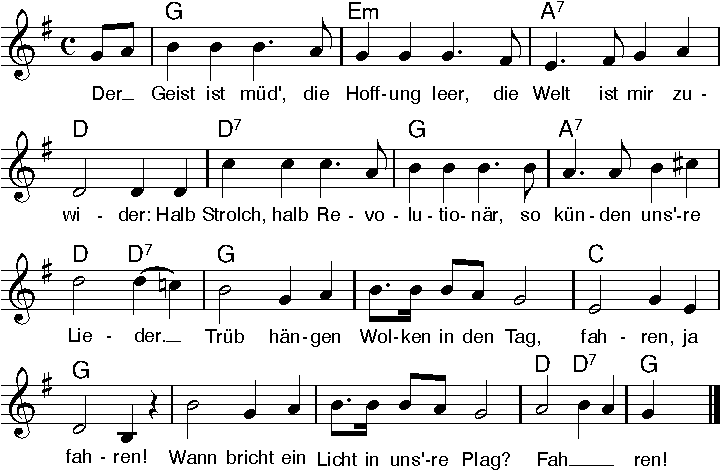
\includegraphics[width=1\textwidth]{Noten/Lied043.pdf}	

\beginverse
Schreit \[G]jeder mir die \[Em]Ohren voll vom \[A7]Paradies auf \[D]Erden.
Weiß \[D7]nicht, wen ich be\[G]dauern soll, weiß \[A7]nur: Es wird nicht \[D]wer\[D7]den.
\endverse

\beginchorus
\[G]Trüb hängen Wolken in den Tag, \[C]fahren, ja \[G]fahren!
Wann bricht ein Licht in uns're Plag? \[D]Fa\[D7]hr\[G]en!
\endchorus

\beginverse
Ein ^Rädchen bin ich ^in der Welt, muss ^mich mitunter ^drehen.
Und ^doch, ihr Herr'n, wem's ^nicht gefällt, mag ^mich von hinten ^se^hen!
\endverse

\printchorus

\beginverse
So ^fahr' ich, weil ich ^leben will das ^Freie, Wunder^bare.
Wer ^Tod mir wünscht, der ^leg' mich still; ich ^lebe, weil ich ^fah^re!
\endverse

\beginchorus
\[G]Trüb hängen Wolken in den Tag, \[C]fahren, ja \[G]fahren!
Licht bricht durch Dunkel wie ein Schlag. \[D]Fa\[D7]hr\[G]en!
\endchorus

\endsong
